%% Please fill in your name and collaboration statement here.
\newcommand{\studentName}{**FILL IN YOUR NAME HERE**}
\newcommand{\collaborationStatement}{**FILL IN YOUR COLLABORATION STATEMENT HERE \\ (See the syllabus for information)**}


%%%%%%%%%%%%%%%%%%%%%%%%%%%%%%%%%%%%%%%%%%%%%%%
\documentclass[solution, letterpaper]{cs20}
\usepackage{enumerate}
\usepackage{tikz}
\usepackage{pgf}
\usepackage{tikz}
\usepackage{hyperref}
\begin{document}
\header{7}{Due Wednesday, March 30, 2016 at 9:59am. All students should submit an electronic copy.}

%%%%%%%%%%%%%%%%%%%%%%%%%%%%%%%%%%%%%%%%%%%%%%%
\PART{Erin}

\problem{4+2}{1/4 page}
\subproblem Prove that in every graph, there are an even number of vertices of odd degree. \emph{Hint: Use the Handshaking Lemma.}
\subproblem Conclude that at a party where some people shake
hands, the number of people who shake hands an odd number of times is an
even number.

\begin{solution} 
\subsolution Partitioning the vertices into those of even degree and those of odd degree, we know
\[
{\sum_{v \in V} d(v)}\ =
\sum_{d(v) \mbox{ {\scriptsize is even}}} d(v)\ +\
\sum_{d(v) \mbox{ {\scriptsize is odd}}} d(v)
\]
By the Handshaking Lemma, the value of the lefthand side of this
equation equals twice the number of edges, and so is even.  The first
summand on the righthand side is even since it is a sum of even
values.  So the second summand on the righthand side must also be even.
But since it is entirely a sum of odd values, it must must contain an even
number of terms.  That is, there must be an even number of vertices with
odd degree.

\subsolution We can represent the people at the party by the vertices of a
graph.  If two people shake hands, then there is an edge between the
corresponding vertices.  So the degree of a vertex is the number of
handshakes the corresponding person performed.  The result in the first
part of this problem now implies that there are an even number of
odd-degree vertices, which translates into an even number of people who
shook an odd number of hands.
\end{solution}

\problem{2+2+2}{1/2 page}
A tree is an undirected graph in which any two vertices are connected by exactly one path (i.e.~a graph with no cycles).  
\subproblem Prove that every tree with at least 2 nodes contains some vertex of degree $1$.
\subproblem Prove for a tree $G=(V,E)$ by induction on $|V|$ that $|E|=|V|-1$.
\subproblem A \emph{spanning tree} of a graph $G=(V,E)$ is a tree on the set of all vertices of $G$ whose edges are in $E$. In other words, it is a tree that connects all the vertices of $G$ using only edges in $G$.  Prove or disprove: For a given a graph $G$, any two spanning trees of $G$ are isomorphic.

\begin{solution}
\subsolution Proof by contradiction. Suppose every node in graph $G$ has degree $\geq 1$. Starting at any vertex $v$, follow a sequence of distinct edges until you see a vertex twice; this is guaranteed to happen because the degree of every vertex is at least two, so upon arriving at a vertex for the first time it is always possible to leave the vertex on another edge (note that here we are assuming a finite graph). When a vertex repeats for the first time, we have discovered a cycle, which contradicts the fact that our graph is a tree.

\subsolution Base Case: In a basic tree (one node), there are zero edges, so the claim holds. 
\begin{itemize}
\item[] Inductive Step: Assume that the predicate holds for $|V|=n.$ Then given a tree on $n+1$ nodes, we can choose some vertex of degree $1$.  Removing this vertex removes one edge, and gives us a tree on $n$ vertices, which has $n-1$ edges by our inductive hypothesis. Thus our original tree had $n$ edges, and by induction we are done.  
\end{itemize}

\subsolution Not true. There are two different spanning trees of the fully connected graph with 4 nodes, for example. One spanning tree has 2 vertices with degree 1 and 2 vertices with degree 2. The other spanning tree has 3 vertices with degree 1 and 1 vertex with degree 3.

\end{solution}

%%%%%%%%%%%%%%%%%%%%%%%%%%%%%%%%%%%%%%%%%%%%%%%
\PART{Hannah}
%%%%%%%%%%%%%%%%%%%%%%%%%%%%%%%%%%%%%%%%%%%%%%%

%% PROBLEM 1 %%
\problem{2+1+3}{}

Below is a graph of some cities and the roads connecting them showing the maximum number of inches of snow that can fall before the roads become impassable. For example, if 2 inches of snow fall, the New York to Albany route remains operational, but if 2.25 inches of snow fall, the road is closed. Snowfall is always uniform everywhere across the region.

\medskip

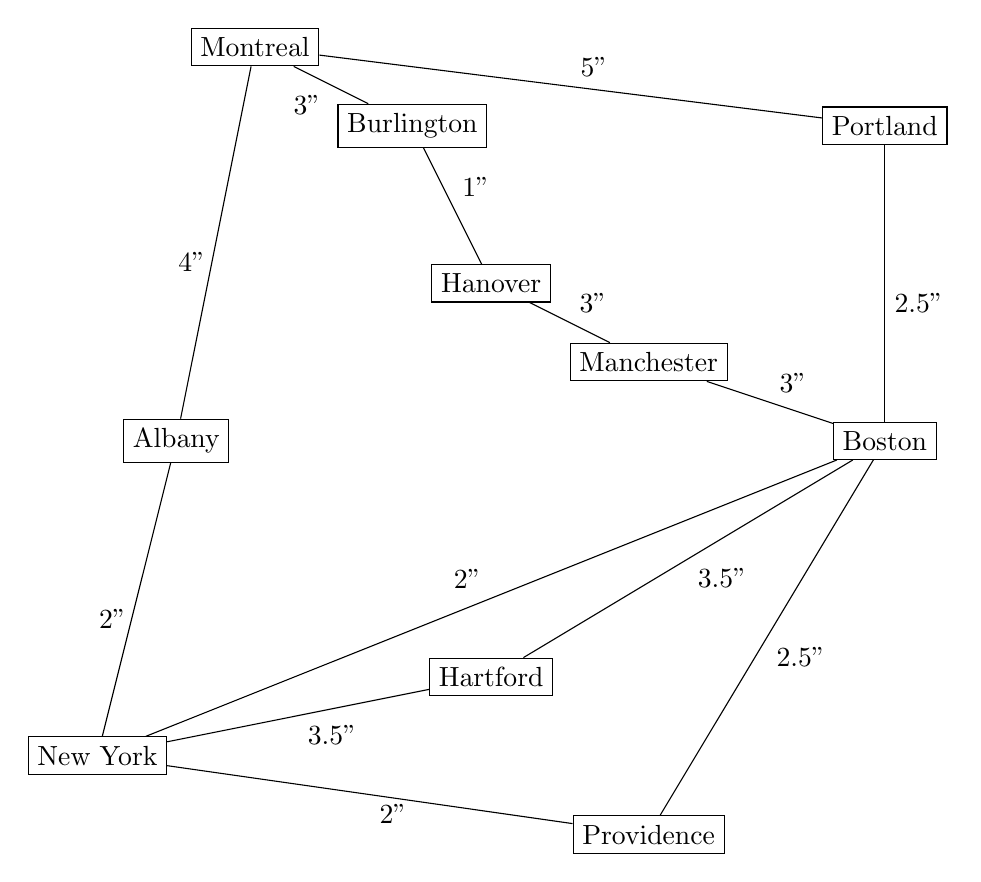
\begin{tikzpicture}
\node (New York) at (-2,0) [shape = rectangle, draw] {New York};

\node (Hartford) at (3, 1) [shape = rectangle, draw] {Hartford};

\node (Providence) at (5, -1) [shape=rectangle, draw] {Providence};

\node (Albany) at (-1,4) [shape=rectangle, draw] {Albany};

\node (Boston) at (8,4) [shape = rectangle, draw] {Boston};

\node (Manchester) at (5,5) [shape=rectangle, draw] {Manchester};

\node (Hanover) at (3, 6) [shape=rectangle, draw] {Hanover};

\node (Burlington) at (2, 8) [shape=rectangle, draw] {Burlington};

\node (Montreal) at (0,9) [shape=rectangle, draw] {Montreal};

\node (Portland) at (8,8) [shape=rectangle, draw] {Portland};


\path [-]   (New York)  edge  node[below left]  {2''}  (Albany)
    edge  node[above left]  {2''}  (Boston)
    edge  node[below right]  {3.5''}  (Hartford)
    edge  node[below right]  {2''}  (Providence)

  (Boston)  edge  node[below right]  {2.5''}  (Portland)
    edge  node[above right]  {3''}  (Manchester)
    edge  node[below right]  {3.5''}  (Hartford)
    edge  node[below right]  {2.5''}  (Providence)

  (Montreal)  edge  node[below left]  {3''}  (Burlington)
    edge  node[below left]  {4''}  (Albany)
    edge  node[above right]  {5''}  (Portland)
  
  (Hanover)  edge  node[above right]  {1''}  (Burlington)
    edge  node[above right]  {3''}  (Manchester);
\end{tikzpicture}

\subproblem Ignoring the labels, what is the edge connectivity of the region? What is the vertex connectivity?

\subproblem Now following the snowfall criterion for edge removal, what is the maximum amount of snowfall that would leave the region connected?

\subproblem Does the graph have any articulation points? Does it have any bridges? How would your answers change if 2 inches of snow fell on the region? Identify the articulation points or bridges if appropriate.

\begin{solution}

  \subsolution The edge connectivity is 2. The vertex connectivity is 2.

  \subsolution The maximum amount of snowfall that would leave the region connected is 2.5 inches.

  \subsolution The graph does not have any articulation points or bridges. If 2 inches of snow fell, Montreal and Manchester would become articulation points and Montreal-Burlington and Burlington-Hanover would become bridges.

\end{solution}

%% PROBLEM 2 %%
\problem{4}{6 lines}
Prove that if an edge is not part of any cycle, then it is a bridge.

\begin{solution}

Suppose an edge $e$ with endpoints $(u,v)$ is not part of any cycle. Since $u$ and $v$ are connected (by $e$), then they are in the same connected component. $e$ is the only path from $u$ to $v$ because if there were any other path $u, x_1, x_2, ... x_i, v$, then there would be a cycle $u, x_1, x_2, ... x_i, v, u$ using $e$. Therefore, if we remove $e$ from the graph, there is no path from $u$ to $v$. This means that $u$ and $v$ are in different connected components. Since $u$ and $v$ were originally in the same connected component, $e$ must be a bridge.

\end{solution}
\end{document}
